
\section{QR Module }
The main idea of this design is to overcome the challenges faced by every national in the bus ticketing system of regional buses. The suggested system consists of an android application with QR Code reader and a money wallet. The android application has an user familiar interface for both the passenger and the conductor to operate, so that it'll be convenient to apply even for people who aren't much educated.
The application consists of separate enrollment for both passenger and conductor. The conductors account enrollment is governed by the admin itself. The admin will give the credentials for conductor so that not everyone can register as conductor. Passenger enrollment is effortless, anyone can register as a passenger with a username and password. Once registered in, both conductor and passenger have to connect their bank account to the application, so that they can transfer, add and withdraw money from the application wallet. While boarding the bus, the passenger has to choose from and to the destination. The bus fare from one spot to another, with the basis of kilometres, is already set by the admin. The fare cost will be shown dynamically on travellers dashboard after choosing destination starting and ending. A QR Code will be generated with this information on the passengers display, which is then scrutinised by the conductor using the QR reader from his account. After surveying, the mentioned bus fare will be debited from the passenger's application and get credited to the conductor’s application wallet. Once the transaction is complete, an acknowledgement will be transferred to the passenger in the form of a text message. The passenger’s and the conductor’s database will get streamlined with trip details. In this way both, passenger and conductor will have a smooth ticketing experience.


\begin{figure}
\centering
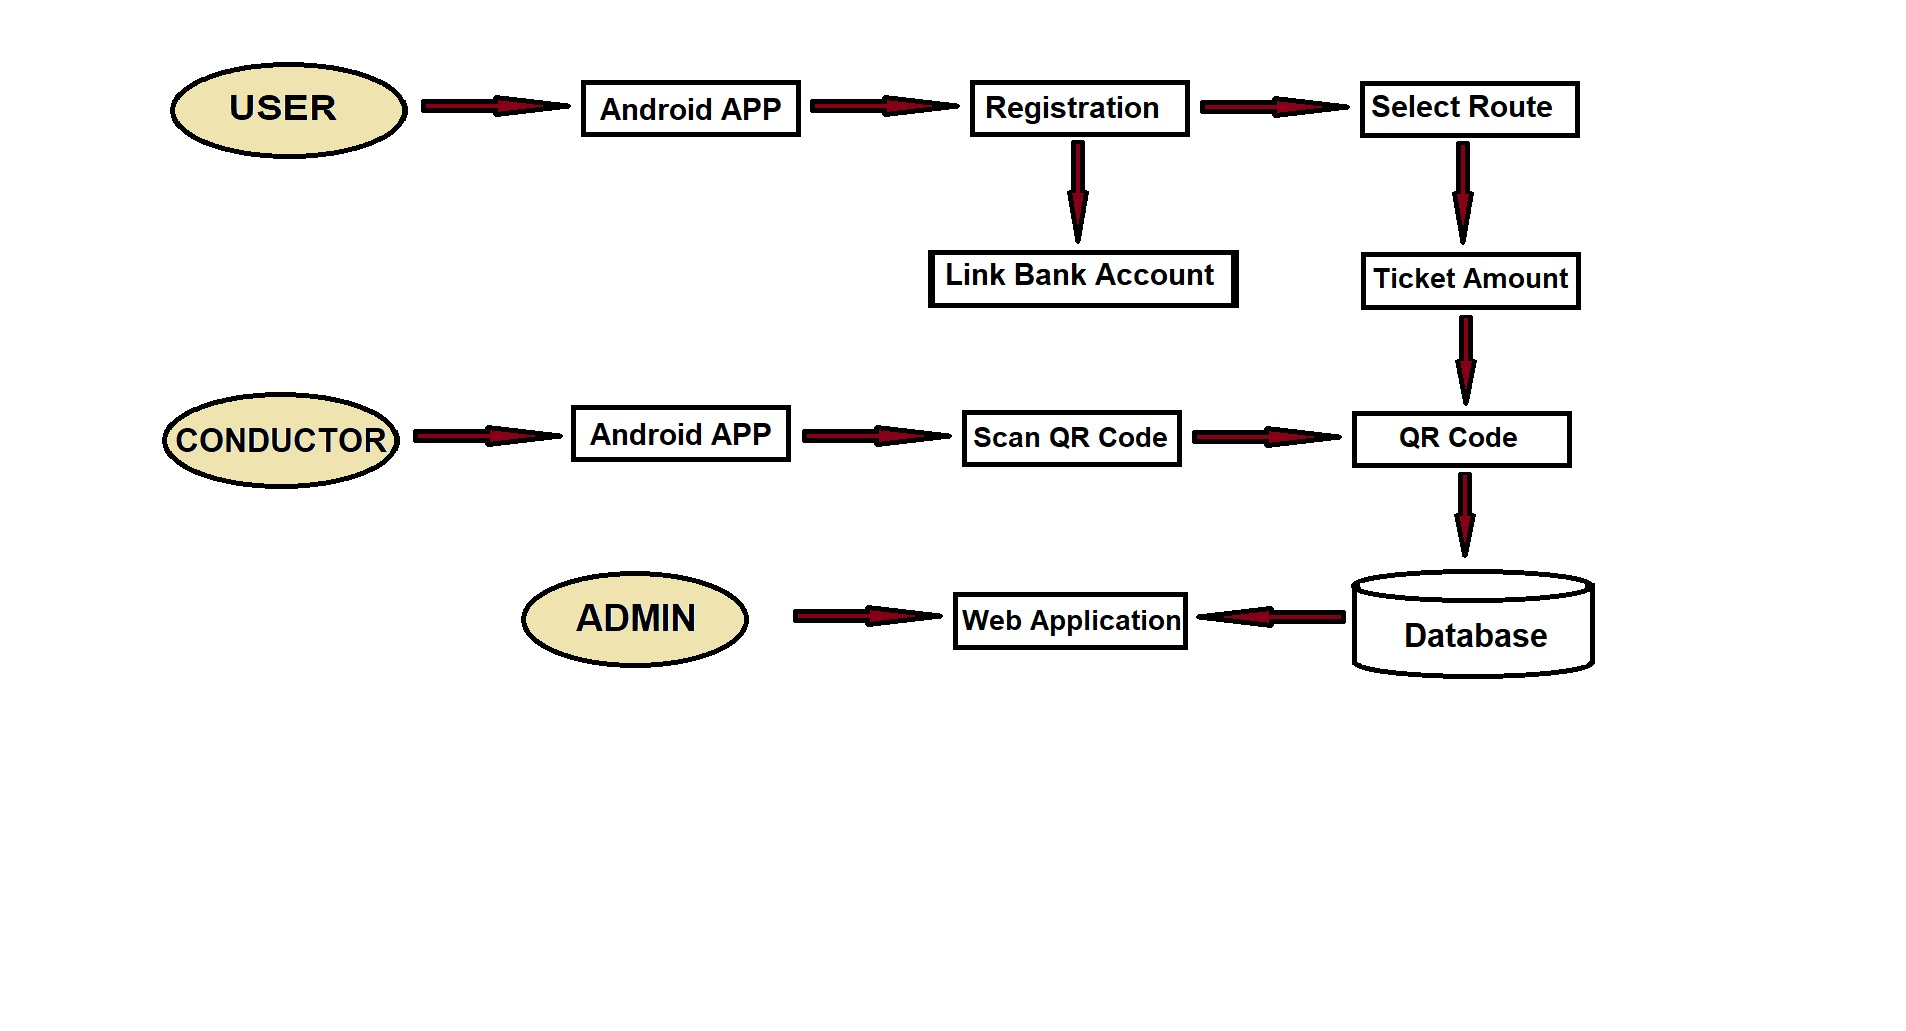
\includegraphics[width=1\textwidth]{Data FLow Diagram of System.jpg}
\caption{Data Flow Diagram Of System}
\end{figure}

\section{ETA and MQTT Module }

The device advanced on this paper objectives to minimise the ready time to board the bus, control and optimise the fleet of buses efficaciously and to offer a actual time facts of the appearance time of the bus. The inputs used are the latitude and longitude extracted from the GPS receiver of the bus. The extracted statistics from the GPS receiver is filled with extra records together with path number, registration number, timestamp and is transmitted to a MQTT broker. The latitude and longitude is processed at the hardware mapped to compute the shortest route the use of Dijkstra`s Algorithm on a predefined listing of bus stops at the path. The region of the bus is likewise up to date to a facts logger maintained in a Google spreadsheet, that acts as a cloud storage. The facts logger serves because the anciental dataset to construct the common time primarily based totally ETA prediction version. The steps of processing are completed in every module as proven withinside the structure diagram proven in Fig. 2. The outputs received after processing the facts in actual time are the ETA to the ultimate stops and the verbal exchange of the function. Based on actual time function updates, dependable facts may be given to commuters and additionally higher tracking of the fleet of buses may be completed.The glide of facts on this environment is illustrated in Fig. 3. The structure diagram and the modules of the whole device are represented in Fig. 2. The region of the bus is captured the use of a GPS receiver.

\begin{figure}
\centering
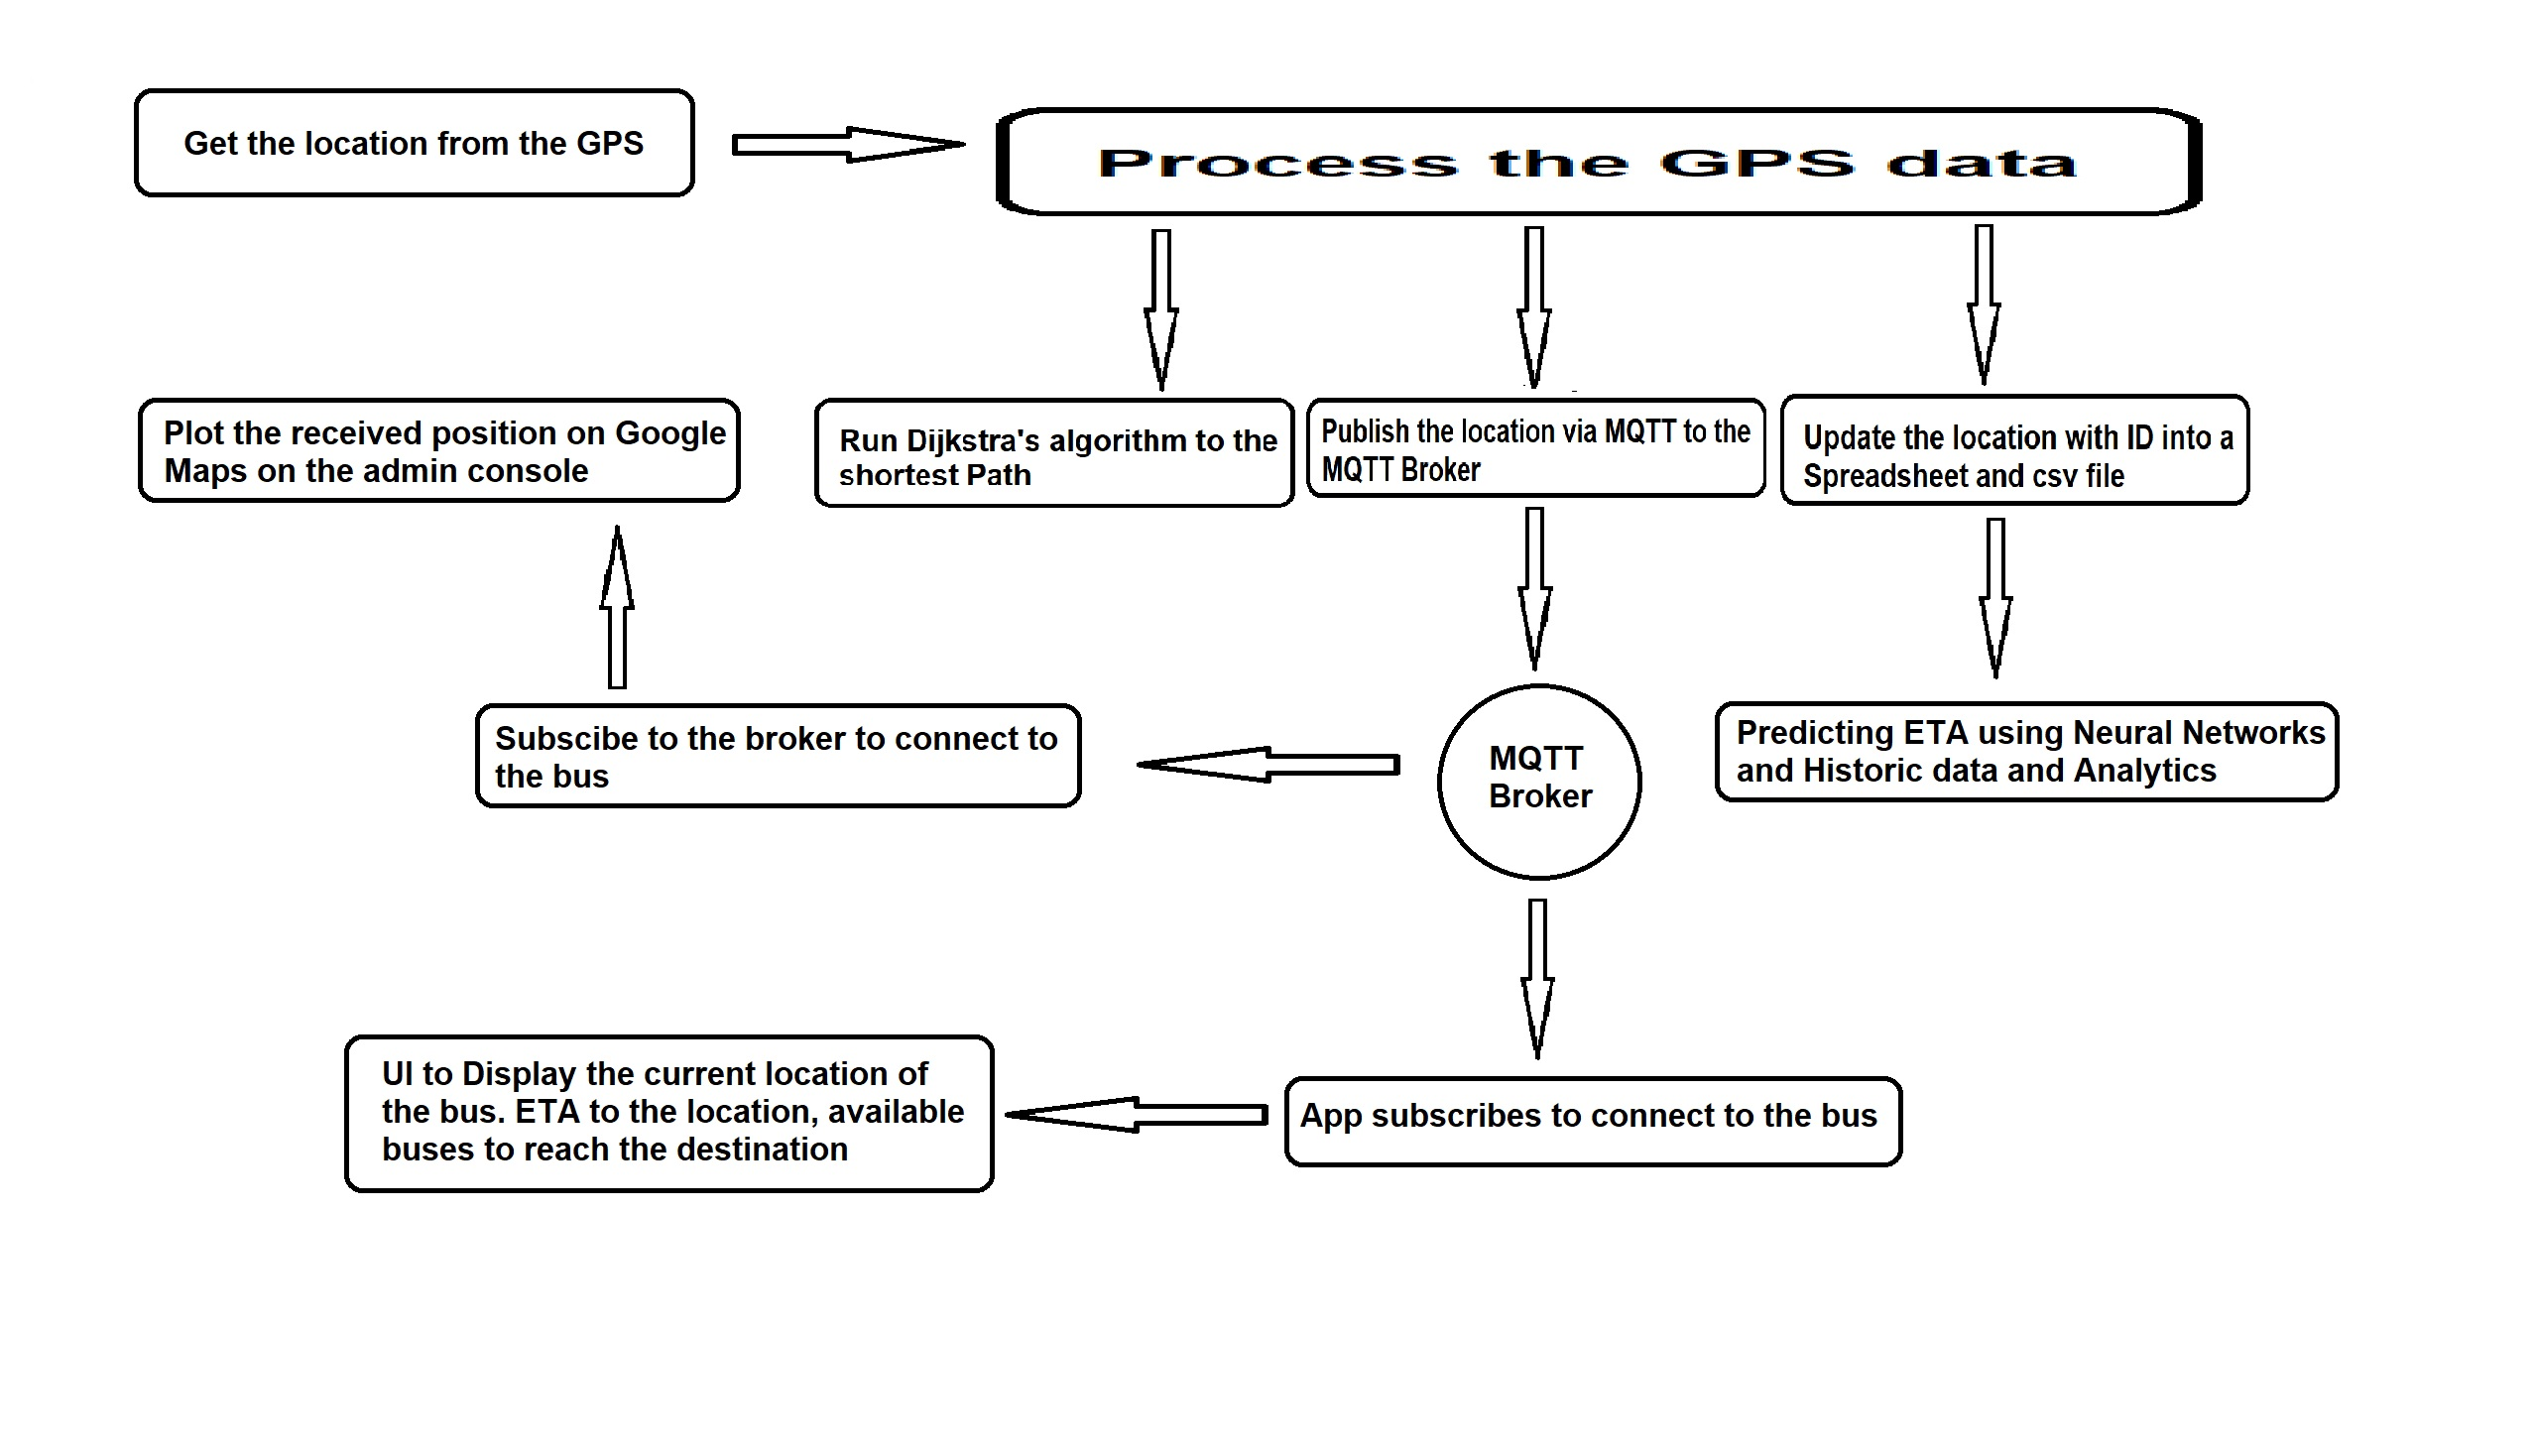
\includegraphics[width=1\textwidth]{Architecture Diagram of The System.jpg}
\caption{Architecture Diagram of The System}
\end{figure}

The data from the GPS is streamed constantly and it contains the Latitude, Longitude, Number of Satellites that the GPS receiver is capable of join to, Deviation or Error withinside the position (in phrases of metres),etc. The facts is cleaned and the Latitude and Longitude is extracted from the data stream. The latitude and longitude are the inputs to the Dijkstra`s Algorithm to compute the shortest distance to the destination (that's preset for the complete journey) from the present day position. To facilitate the capacity to file and save the motion of every bus, a data logger is designed. The information logger periodically populates a Google spreadsheet and a CSV record with the timestamp, registration number, call of the driver, destination and location of the bus. The use of Google Sheets is a cost-powerful technique and saves time putting in a custom cloud infrastructure. A csv record is maintained onboard the hardware at the bus. The cause of the csv record is to usher in redundancy to prevent data loss or data corruption and it acts just like the black box in aircraft. Each bus is related to a unique, particular subject matter (registration no.). A subject matter is the parameter in MQTT that's used to push/fetch the correct contents from the MQTT dealer. This makes certain that a quick scalability of the prototype is possible. A prediction version primarily based totally at the historic facts is constructed to estimate the appearance time of the bus to any precise stop at the route. The bus may be monitored in actual time with the aid of using the administrator the use of a easy internet application. The commuter makes use of the proposed app to get actual-time facts in regards to the modern-day region of the bus and an Estimated Arrival Time to his/her stop.The utilization sample of the proposed application is upto the user`s discretion as as soon as the app is attached to the MQTT broker the essential data could be available with the app.


\begin{figure}
\centering
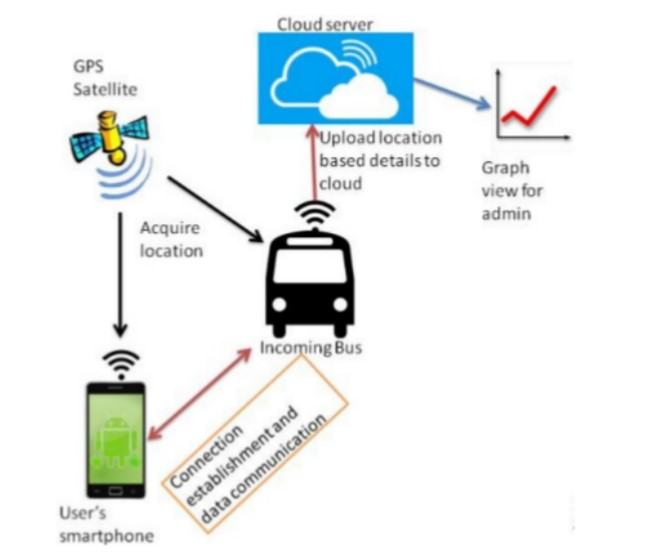
\includegraphics[width=1\textwidth]{overview.jpg}
\caption{An Overview of the data flow in the system}
\end{figure}
